\documentclass{standalone}
\usepackage{tikz}
\usetikzlibrary{patterns, positioning}

\begin{document}
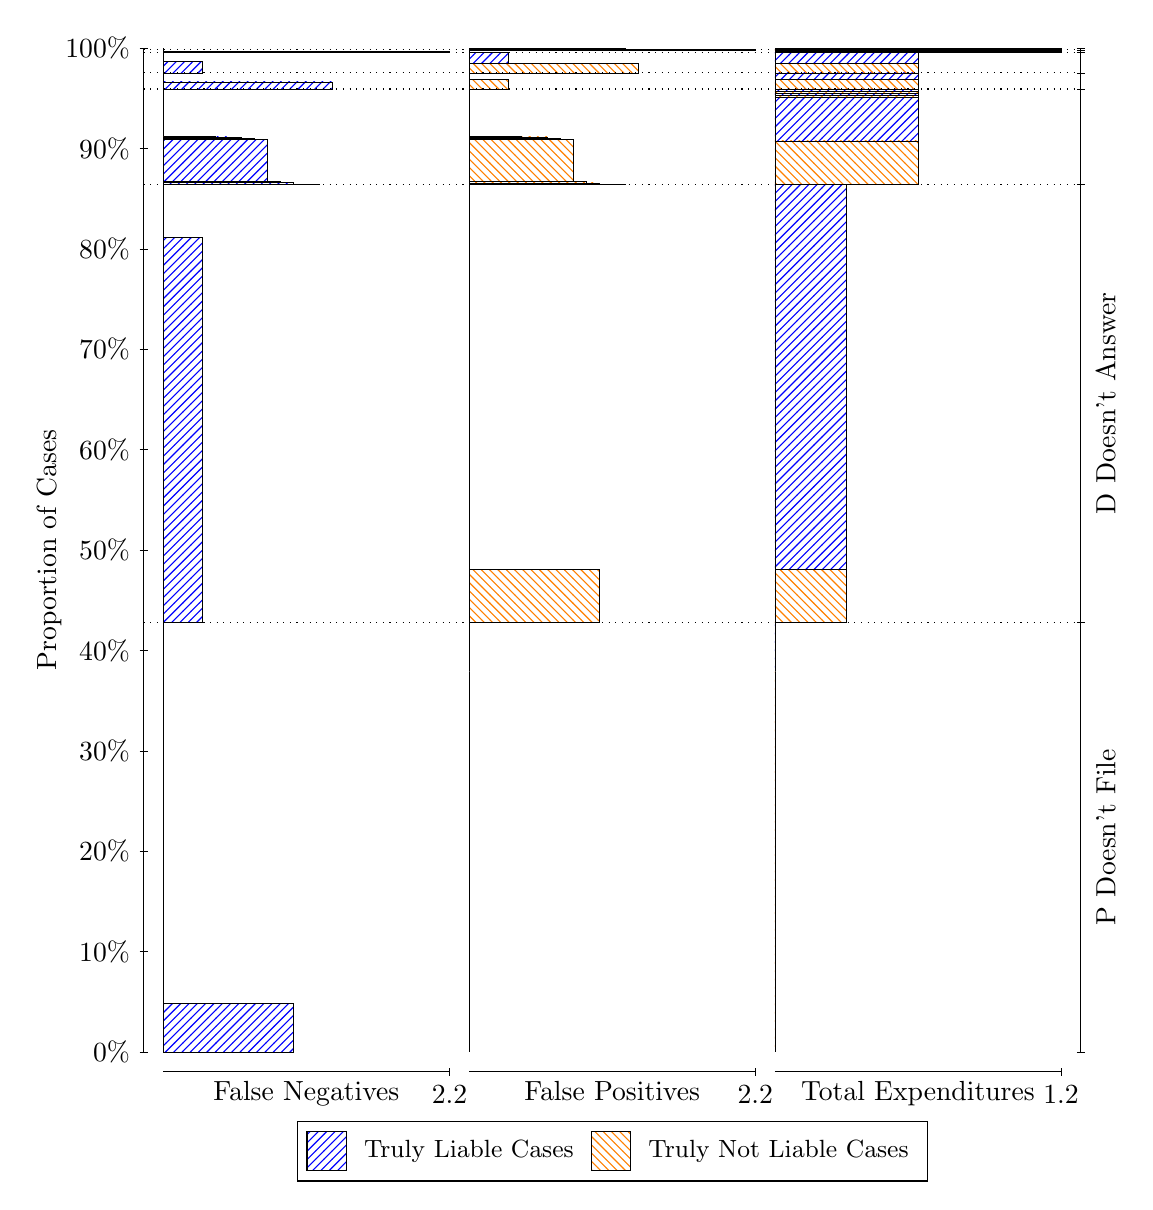
\begin{tikzpicture}
\draw[black, very thin] (1.5,1.75) -- (1.5,14.5);
\node[rotate=90, anchor=center] at (0.3, 8.125) {Proportion of Cases};
\draw[black, very thin] (1.45,1.75) -- (1.55,1.75);
\node[anchor=east] at (1.45, 1.75) {0\%};
\draw[black, very thin] (1.45,3.025) -- (1.55,3.025);
\node[anchor=east] at (1.45, 3.025) {10\%};
\draw[black, very thin] (1.45,4.3) -- (1.55,4.3);
\node[anchor=east] at (1.45, 4.3) {20\%};
\draw[black, very thin] (1.45,5.575) -- (1.55,5.575);
\node[anchor=east] at (1.45, 5.575) {30\%};
\draw[black, very thin] (1.45,6.85) -- (1.55,6.85);
\node[anchor=east] at (1.45, 6.85) {40\%};
\draw[black, very thin] (1.45,8.125) -- (1.55,8.125);
\node[anchor=east] at (1.45, 8.125) {50\%};
\draw[black, very thin] (1.45,9.4) -- (1.55,9.4);
\node[anchor=east] at (1.45, 9.4) {60\%};
\draw[black, very thin] (1.45,10.675) -- (1.55,10.675);
\node[anchor=east] at (1.45, 10.675) {70\%};
\draw[black, very thin] (1.45,11.95) -- (1.55,11.95);
\node[anchor=east] at (1.45, 11.95) {80\%};
\draw[black, very thin] (1.45,13.225) -- (1.55,13.225);
\node[anchor=east] at (1.45, 13.225) {90\%};
\draw[black, very thin] (1.45,14.5) -- (1.55,14.5);
\node[anchor=east] at (1.45, 14.5) {100\%};

\draw[black, very thin] (13.4,1.75) -- (13.4,14.5);
\draw[black, very thin] (13.35,1.75) -- (13.45,1.75);
\node[anchor=west] at (13.35, 1.75) {};
\draw[black, very thin] (13.35,7.2066) -- (13.45,7.2066);
\node[anchor=west] at (13.35, 7.2066) {};
\draw[black, very thin] (13.35,12.77) -- (13.45,12.77);
\node[anchor=west] at (13.35, 12.77) {};
\draw[black, very thin] (13.35,13.98) -- (13.45,13.98);
\node[anchor=west] at (13.35, 13.98) {};
\draw[black, very thin] (13.35,14.185) -- (13.45,14.185);
\node[anchor=west] at (13.35, 14.185) {};
\draw[black, very thin] (13.35,14.447) -- (13.45,14.447);
\node[anchor=west] at (13.35, 14.447) {};
\draw[black, very thin] (13.35,14.476) -- (13.45,14.476);
\node[anchor=west] at (13.35, 14.476) {};
\draw[black, very thin] (13.35,14.5) -- (13.45,14.5);
\node[anchor=west] at (13.35, 14.5) {};

\draw[black, very thin, pattern color=blue, pattern=north east lines] (1.75,1.75) rectangle (3.4015,2.3717);
\draw[black, very thin, pattern color=orange, pattern=north west lines] (1.75,2.3717) rectangle (1.75,7.2066);
\draw[black, very thin, pattern color=blue, pattern=north east lines] (1.75,7.2066) rectangle (2.2455,12.099);
\draw[black, very thin, pattern color=orange, pattern=north west lines] (1.75,12.099) rectangle (1.75,12.77);
\draw[black, very thin, pattern color=blue, pattern=north east lines] (1.75,12.77) rectangle (3.7318,12.772);
\draw[black, very thin, pattern color=blue, pattern=north east lines] (1.75,12.772) rectangle (3.5667,12.773);
\draw[black, very thin, pattern color=blue, pattern=north east lines] (1.75,12.773) rectangle (3.4015,12.791);
\draw[black, very thin, pattern color=blue, pattern=north east lines] (1.75,12.791) rectangle (3.2364,12.791);
\draw[black, very thin, pattern color=blue, pattern=north east lines] (1.75,12.791) rectangle (3.2364,12.804);
\draw[black, very thin, pattern color=blue, pattern=north east lines] (1.75,12.804) rectangle (3.0712,13.34);
\draw[black, very thin, pattern color=blue, pattern=north east lines] (1.75,13.34) rectangle (2.9061,13.354);
\draw[black, very thin, pattern color=blue, pattern=north east lines] (1.75,13.354) rectangle (2.7409,13.37);
\draw[black, very thin, pattern color=blue, pattern=north east lines] (1.75,13.37) rectangle (2.5758,13.371);
\draw[black, very thin, pattern color=blue, pattern=north east lines] (1.75,13.371) rectangle (2.4106,13.374);
\draw[black, very thin, pattern color=orange, pattern=north west lines] (1.75,13.374) rectangle (1.75,13.98);
\draw[black, very thin, pattern color=blue, pattern=north east lines] (1.75,13.98) rectangle (3.897,14.069);
\draw[black, very thin, pattern color=orange, pattern=north west lines] (1.75,14.069) rectangle (1.75,14.185);
\draw[black, very thin, pattern color=blue, pattern=north east lines] (1.75,14.185) rectangle (2.2455,14.329);
\draw[black, very thin, pattern color=orange, pattern=north west lines] (1.75,14.329) rectangle (1.75,14.447);
\draw[black, very thin, pattern color=blue, pattern=north east lines] (1.75,14.447) rectangle (5.3833,14.458);
\draw[black, very thin, pattern color=orange, pattern=north west lines] (1.75,14.458) rectangle (1.75,14.476);
\draw[black, very thin, pattern color=orange, pattern=north west lines] (1.75,14.476) rectangle (1.75,14.486);
\draw[black, very thin, pattern color=blue, pattern=north east lines] (1.75,14.486) rectangle (1.75,14.5);
\draw[black, very thin, pattern color=orange, pattern=north west lines] (5.6333,1.75) rectangle (5.6333,6.5849);
\draw[black, very thin, pattern color=blue, pattern=north east lines] (5.6333,6.5849) rectangle (5.6333,7.2066);
\draw[black, very thin, pattern color=orange, pattern=north west lines] (5.6333,7.2066) rectangle (7.2848,7.8774);
\draw[black, very thin, pattern color=blue, pattern=north east lines] (5.6333,7.8774) rectangle (5.6333,12.77);
\draw[black, very thin, pattern color=orange, pattern=north west lines] (5.6333,12.77) rectangle (7.6152,12.772);
\draw[black, very thin, pattern color=orange, pattern=north west lines] (5.6333,12.772) rectangle (7.45,12.773);
\draw[black, very thin, pattern color=orange, pattern=north west lines] (5.6333,12.773) rectangle (7.2848,12.788);
\draw[black, very thin, pattern color=orange, pattern=north west lines] (5.6333,12.788) rectangle (7.1197,12.803);
\draw[black, very thin, pattern color=orange, pattern=north west lines] (5.6333,12.803) rectangle (6.9545,13.339);
\draw[black, very thin, pattern color=orange, pattern=north west lines] (5.6333,13.339) rectangle (6.7894,13.352);
\draw[black, very thin, pattern color=orange, pattern=north west lines] (5.6333,13.352) rectangle (6.6242,13.371);
\draw[black, very thin, pattern color=orange, pattern=north west lines] (5.6333,13.371) rectangle (6.4591,13.372);
\draw[black, very thin, pattern color=orange, pattern=north west lines] (5.6333,13.372) rectangle (6.2939,13.376);
\draw[black, very thin, pattern color=blue, pattern=north east lines] (5.6333,13.376) rectangle (5.9636,13.379);
\draw[black, very thin, pattern color=blue, pattern=north east lines] (5.6333,13.379) rectangle (5.7985,13.38);
\draw[black, very thin, pattern color=blue, pattern=north east lines] (5.6333,13.38) rectangle (5.6333,13.98);
\draw[black, very thin, pattern color=orange, pattern=north west lines] (5.6333,13.98) rectangle (6.1288,14.097);
\draw[black, very thin, pattern color=blue, pattern=north east lines] (5.6333,14.097) rectangle (5.6333,14.185);
\draw[black, very thin, pattern color=orange, pattern=north west lines] (5.6333,14.185) rectangle (7.7803,14.303);
\draw[black, very thin, pattern color=blue, pattern=north east lines] (5.6333,14.303) rectangle (6.1288,14.447);
\draw[black, very thin, pattern color=orange, pattern=north west lines] (5.6333,14.447) rectangle (5.6333,14.465);
\draw[black, very thin, pattern color=blue, pattern=north east lines] (5.6333,14.465) rectangle (5.6333,14.476);
\draw[black, very thin, pattern color=orange, pattern=north west lines] (5.6333,14.476) rectangle (9.2667,14.486);
\draw[black, very thin, pattern color=blue, pattern=north east lines] (5.6333,14.486) rectangle (7.6152,14.5);
\draw[black, very thin, pattern color=orange, pattern=north west lines] (9.5167,1.75) rectangle (9.5167,6.5849);
\draw[black, very thin, pattern color=blue, pattern=north east lines] (9.5167,6.5849) rectangle (9.5167,7.2066);
\draw[black, very thin, pattern color=orange, pattern=north west lines] (9.5167,7.2066) rectangle (10.425,7.8774);
\draw[black, very thin, pattern color=blue, pattern=north east lines] (9.5167,7.8774) rectangle (10.425,12.77);
\draw[black, very thin, pattern color=orange, pattern=north west lines] (9.5167,12.77) rectangle (11.333,13.322);
\draw[black, very thin, pattern color=blue, pattern=north east lines] (9.5167,13.322) rectangle (11.333,13.874);
\draw[black, very thin, pattern color=orange, pattern=north west lines] (9.5167,13.874) rectangle (11.333,13.899);
\draw[black, very thin, pattern color=blue, pattern=north east lines] (9.5167,13.899) rectangle (11.333,13.921);
\draw[black, very thin, pattern color=orange, pattern=north west lines] (9.5167,13.921) rectangle (11.333,13.951);
\draw[black, very thin, pattern color=blue, pattern=north east lines] (9.5167,13.951) rectangle (11.333,13.98);
\draw[black, very thin, pattern color=orange, pattern=north west lines] (9.5167,13.98) rectangle (11.333,14.097);
\draw[black, very thin, pattern color=blue, pattern=north east lines] (9.5167,14.097) rectangle (11.333,14.185);
\draw[black, very thin, pattern color=orange, pattern=north west lines] (9.5167,14.185) rectangle (11.333,14.303);
\draw[black, very thin, pattern color=blue, pattern=north east lines] (9.5167,14.303) rectangle (11.333,14.447);
\draw[black, very thin, pattern color=orange, pattern=north west lines] (9.5167,14.447) rectangle (13.15,14.465);
\draw[black, very thin, pattern color=blue, pattern=north east lines] (9.5167,14.465) rectangle (13.15,14.476);
\draw[black, very thin, pattern color=orange, pattern=north west lines] (9.5167,14.476) rectangle (13.15,14.486);
\draw[black, very thin, pattern color=blue, pattern=north east lines] (9.5167,14.486) rectangle (13.15,14.5);
\draw[black, dotted] (1.5,7.2066) -- (13.4,7.2066);
\draw[black, dotted] (1.5,12.77) -- (13.4,12.77);
\draw[black, dotted] (1.5,13.98) -- (13.4,13.98);
\draw[black, dotted] (1.5,14.185) -- (13.4,14.185);
\draw[black, dotted] (1.5,14.447) -- (13.4,14.447);
\draw[black, dotted] (1.5,14.476) -- (13.4,14.476);
\draw[black, very thin] (1.75,1.5) -- (5.3833,1.5);
\node[anchor=north] at (3.5667, 1.5) {False Negatives};
\draw[black, very thin] (5.3833,1.45) -- (5.3833,1.55);
\node[anchor=north] at (5.3833, 1.45) {2.2};

\draw[black, very thin] (5.6333,1.5) -- (9.2667,1.5);
\node[anchor=north] at (7.45, 1.5) {False Positives};
\draw[black, very thin] (9.2667,1.45) -- (9.2667,1.55);
\node[anchor=north] at (9.2667, 1.45) {2.2};

\draw[black, very thin] (9.5167,1.5) -- (13.15,1.5);
\node[anchor=north] at (11.333, 1.5) {Total Expenditures};
\draw[black, very thin] (13.15,1.45) -- (13.15,1.55);
\node[anchor=north] at (13.15, 1.45) {1.2};

\node[black, centered, rotate=90] at (13.72, 4.4783) {P Doesn't File};
\node[black, centered, rotate=90] at (13.72, 9.9881) {D Doesn't Answer};






\draw (7.449999999999999,1.5) node[draw=none] (baseCoordinate) {};
\begin{scope}[align=center]
        \matrix[scale=0.5, draw=black, below=0.5cm of baseCoordinate, nodes={draw}, column sep=0.1cm]{
            \node[rectangle, draw, minimum width=0.5cm, minimum height=0.5cm, pattern=north east lines, pattern color=blue] {}; &
            \node[draw=none, font=\small] (B) {Truly Liable Cases}; &
            \node[rectangle, draw, minimum width=0.5cm, minimum height=0.5cm, pattern=north west lines, pattern color=orange] {}; &
            \node[draw=none, font=\small] (B) {Truly Not Liable Cases}; \\
            };
\end{scope}

\end{tikzpicture}
\end{document}